\documentclass{oci}
\usepackage[utf8]{inputenc}
\usepackage{lipsum}
\usepackage{tikz}
\usepackage{amsmath}

\title{Viaje a la playa}

\begin{document}
\begin{problemDescription}
David está organizando una salida a la playa con sus amigos. Su ciudad puede ser representada por una grilla de $n$ filas y $m$ columnas. Llamemos a la celda en la $i$-ésima fila y $j$-ésima columna $(i,j)$. El viaje parte en la esquina superior izquierda $(1,1)$ y termina en la esquina inferior derecha $(n,m)$. Desde cada casilla solo se puede pasar a las casillas que compartan un lado.

Cada celda tiene un color asociado a ella, este color es representado por un número $C_{(i,j)}$ que va entre $1$ y $k$. Para tener un viaje agradable se tiene que cumplir una condición: dos casillas consecutivas del viaje no pueden tener el mismo color. Esto significa que si en el viaje se pasa de la casilla $(i_1,j_1)$ a $(i_2,j_2)$ entonces $C_{(i_1,j_1)} \neq C_{(i_2,j_2)}$.

David está muy confundido al ver el mapa y necesita tu ayuda. Tienes que ver si existe un camino agradable y, si existe, imprimir la distancia del camino agradable más corto que lleve a la playa.

Por ejemplo, un mapa posible con $n = 3$, $m = 3$ y $k = 3$ es:

\begin{gather*}
1\ 2\ 1\\
3\ 3\ 2\\
3\ 3\ 1
\end{gather*}

que podríamos representar de la siguiente manera:

\begin{figure}[!h]
\centering
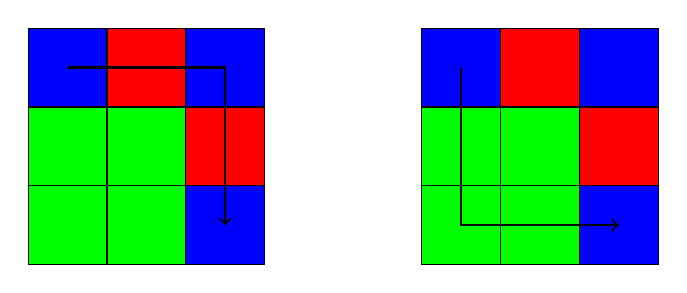
\begin{tikzpicture}
\fill[blue,draw=black] (0,0) rectangle (1,1); \fill[red,draw=black] (1,0) rectangle (2,1); \fill[blue,draw=black] (2,0) rectangle (3,1);
\fill[green,draw=black] (0,0) rectangle (1,-1); \fill[green,draw=black] (1,0) rectangle (2,-1); \fill[red,draw=black] (2,0) rectangle (3,-1);
\fill[green,draw=black] (0,-2) rectangle (1,-1); \fill[green,draw=black] (1,-2) rectangle (2,-1); \fill[blue,draw=black] (2,-2) rectangle (3,-1);
\draw[thick,->] (0.5,0.5) -- (2.5,0.5) -- (2.5,-1.5);

\fill[blue,draw=black] (5,0) rectangle (6,1); \fill[red,draw=black] (6,0) rectangle (7,1); \fill[blue,draw=black] (7,0) rectangle (8,1);
\fill[green,draw=black] (5,0) rectangle (6,-1); \fill[green,draw=black] (6,0) rectangle (7,-1); \fill[red,draw=black] (7,0) rectangle (8,-1);
\fill[green,draw=black] (5,-2) rectangle (6,-1); \fill[green,draw=black] (6,-2) rectangle (7,-1); \fill[blue,draw=black] (7,-2) rectangle (8,-1);
\draw[thick,->] (5.5,0.5) -- (5.5,-1.5) -- (7.5,-1.5);
\end{tikzpicture}
\end{figure}

Aquí mostramos dos caminos posibles que van desde $(1,1)$ hasta $(3,3)$: el izquierdo es agradable pero el derecho no lo es ya que la segunda, tercera y cuarta casilla son del mismo color. La distancia en ambos caminos es $4$.

\end{problemDescription}


\begin{inputDescription}
La primera línea contiene tres enteros $n, m$ y $k$ ($1 \leq n, m \leq 1000$, $2 \leq n*m \leq 10^5$ y $2 \leq k \leq n*m$) que corresponden a las dimensiones de la ciudad y la cantidad de colores que hay.

A continuación siguen $n$ líneas, cada una con $m$ enteros que van entre $1$ y $k$. El $j$-ésimo entero de la $i$-ésima línea representa a $C_{(i,j)}$, el color de la celda $(i,j)$.

\end{inputDescription}

\begin{outputDescription}
Imprime la distancia del camino agradable más corto, si este no existe imprime -1.

\end{outputDescription}

\begin{scoreDescription}
  \subtask{20}
  Se probaran varios casos en que $n = 1$, es decir, el mapa es solo una fila.
  \subtask{20}
  Se probaran varios casos en que $n = 2$ y $k = 2$, es decir, son dos filas con solo dos colores.
  \subtask{20}
  Se probaran varios casos en que $n = 2$.
  \subtask{40}
  Se probaran varios casos sin más restricciones.
\end{scoreDescription}

\begin{sampleDescription}
\sampleIO{sample-1}
\sampleIO{sample-2}
\end{sampleDescription}

\end{document}
